\documentclass{article}
\usepackage{graphicx}
\usepackage[utf8]{inputenc}
\usepackage[vmargin=3.25cm,hmargin=3.25cm]{geometry}
\usepackage{hyperref}
\usepackage{caption}
\usepackage{subcaption}

\title{Finding Breakpoints and Similarity of Viral Genomes using recan}
\author{Abinu Ajithan Jyothini}
\date{August 6th 2020}
\begin{document}
\maketitle
\section{Introduction}
In many different group of viruses recombination of genetic material is an important evolutionary process that generates much of genetic diversity.The patterns of recombination evident within the genomes of viruses can reveal lots of detail about their evolution and biology.Recombination is responsible for the evolution of viruses in response to selective forces present in a host environment \cite{perez2015recombination}. A better understanding of recombination events taking place in the genomes of viruses are useful for gaining in-sites about the biology of the viruses.The patterns of sequence exchange between viruses in different species can reveal otherwise undetectable ecological links between some species and barriers between others.\cite{martin2015rdp4}. The breakpoints of genomes can reveal details about mechanistic and biochemical processes regarding the recombination process.\cite{martin2015rdp4}.This project makes use of the python package 'recan'\cite{babin2020recan}(recombination analyzer) for constructing genetic distance plots and exploring them.Also, we make use of bio-python\cite{chapman2000biopython} package for plotting fasta sequences.
\section{Methods:}
\subsection{recan Python Package:}
recan is a python package developed for the recombination analysis and it provides a mean for constructing genetic distance plots and exploring them interactively.recan is based on python packages like Biopython, Pandas, Matplotlib, and Plotly libraries.recan requires the input to be in the form of alligned fasta sequence.There are options for changing the window size,adjusting the sequence of interest(for example; sequence where the breakpoints occurs), changing the method of distance calculations etc.
\subsection{Input Data:}
The fasta sequence of viral genomes can be obtained from any of the protein data banks. RCSB protein data bank \cite{rose2016rcsb}(https://www.rcsb.org/) is most popular among bioinformatic  scientists.  We can directly obtain the fasta sequence of the genome from RCSB.Since the recan only takes aligned fasta format of the genome, the fasta sequence downloaded from the RCSB protein data bank needs to be alligned.This can be achieved by using NCBI Multiple SEquence Allignment Viewer(https://www.ncbi.nlm.nih.gov/projects/msaviewer/).In this project, i chose lumky skin disease virus's genome \cite{sprygin2018epidemiological} for finding out the breakpoints. I have also used the genome sequence of BCRA1 genes, which are the genes that produce tumor suppressor proteins, for demonstrating the visualization of the fasta sequence.

\section{Results and Discussion:}
\subsection{Breakpoints:}
In genetics, the rearrangement of chromosomes is called mutation.It is an abnormality in the chromosome involving a change in the native chromosome  \cite{zhao2012genome}.Theses changes may involve  several events such as, duplication, inversion, deletion and translocation.These events are usually caused by a breakage in the helices of DNA and rejoining of the broken ends to form a new gene,different from the gene order of the chromosomes before they were broken \cite{griffiths2002modern}.Some regions of chromosomes are more susceptible for rearrangements than others and thus are sources of genetic diseases and cancer.The Figure\ref{Figure:1} shows the breakpoints of lumky skin disease viral genome. We can see that, the recombination breakpoints are at around nucleotide number 1500 and at 1800. This is the clear evidence that recombination is taking place and the genome is undergoing mutation.

\begin{figure}
    \centering
    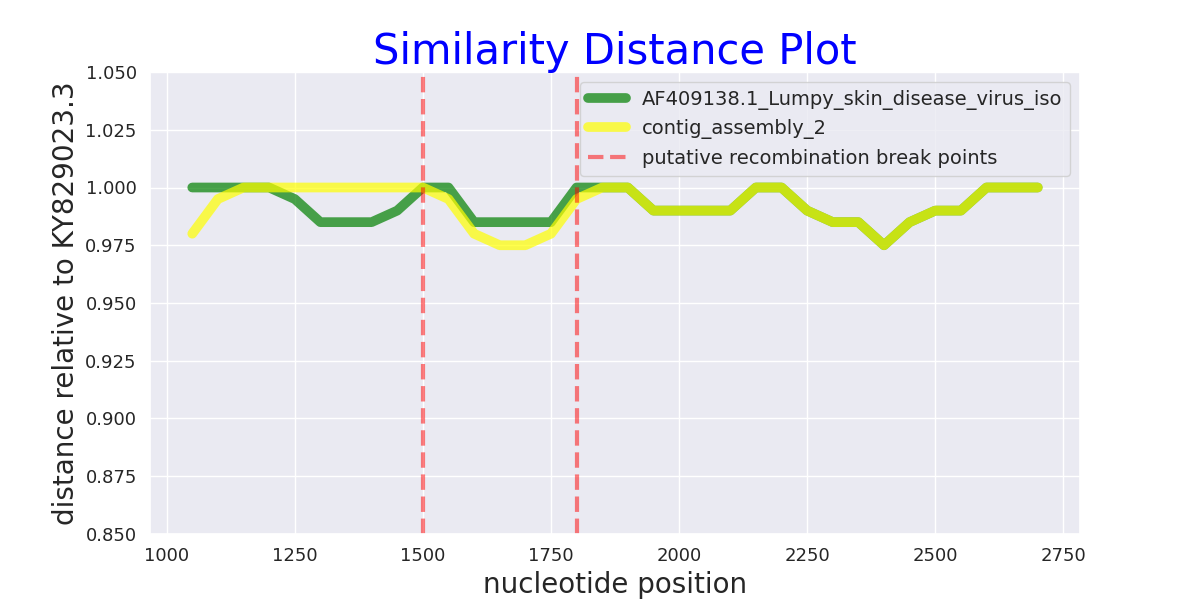
\includegraphics[width=1.2\textwidth]{distance_plot}
    \caption{Distance Plot}
    \label{Figure:1}
\end{figure}

\subsubsection{Breakpoints of HIV sequences:}
I plotted the distance plots of 18 sequences of HIV virus and found out the breakpoints.The subplots shown in Figure\ref{Figure:2} the breakpoints of nine compared sequences.The breakpoints obtained are summarised in Table\ref{Table:1}

\subsubsection{Breakpoints of NoroVirus sequences:}
I have also plotted the distance plots of noro virus genome sequence for finding the breakpoints.Figure\ref{Figure:3} shows the distance plots for noro virus sequence. The breakpoints obtained are given in Table\ref{Table:2}

\begin{figure}
    \centering
    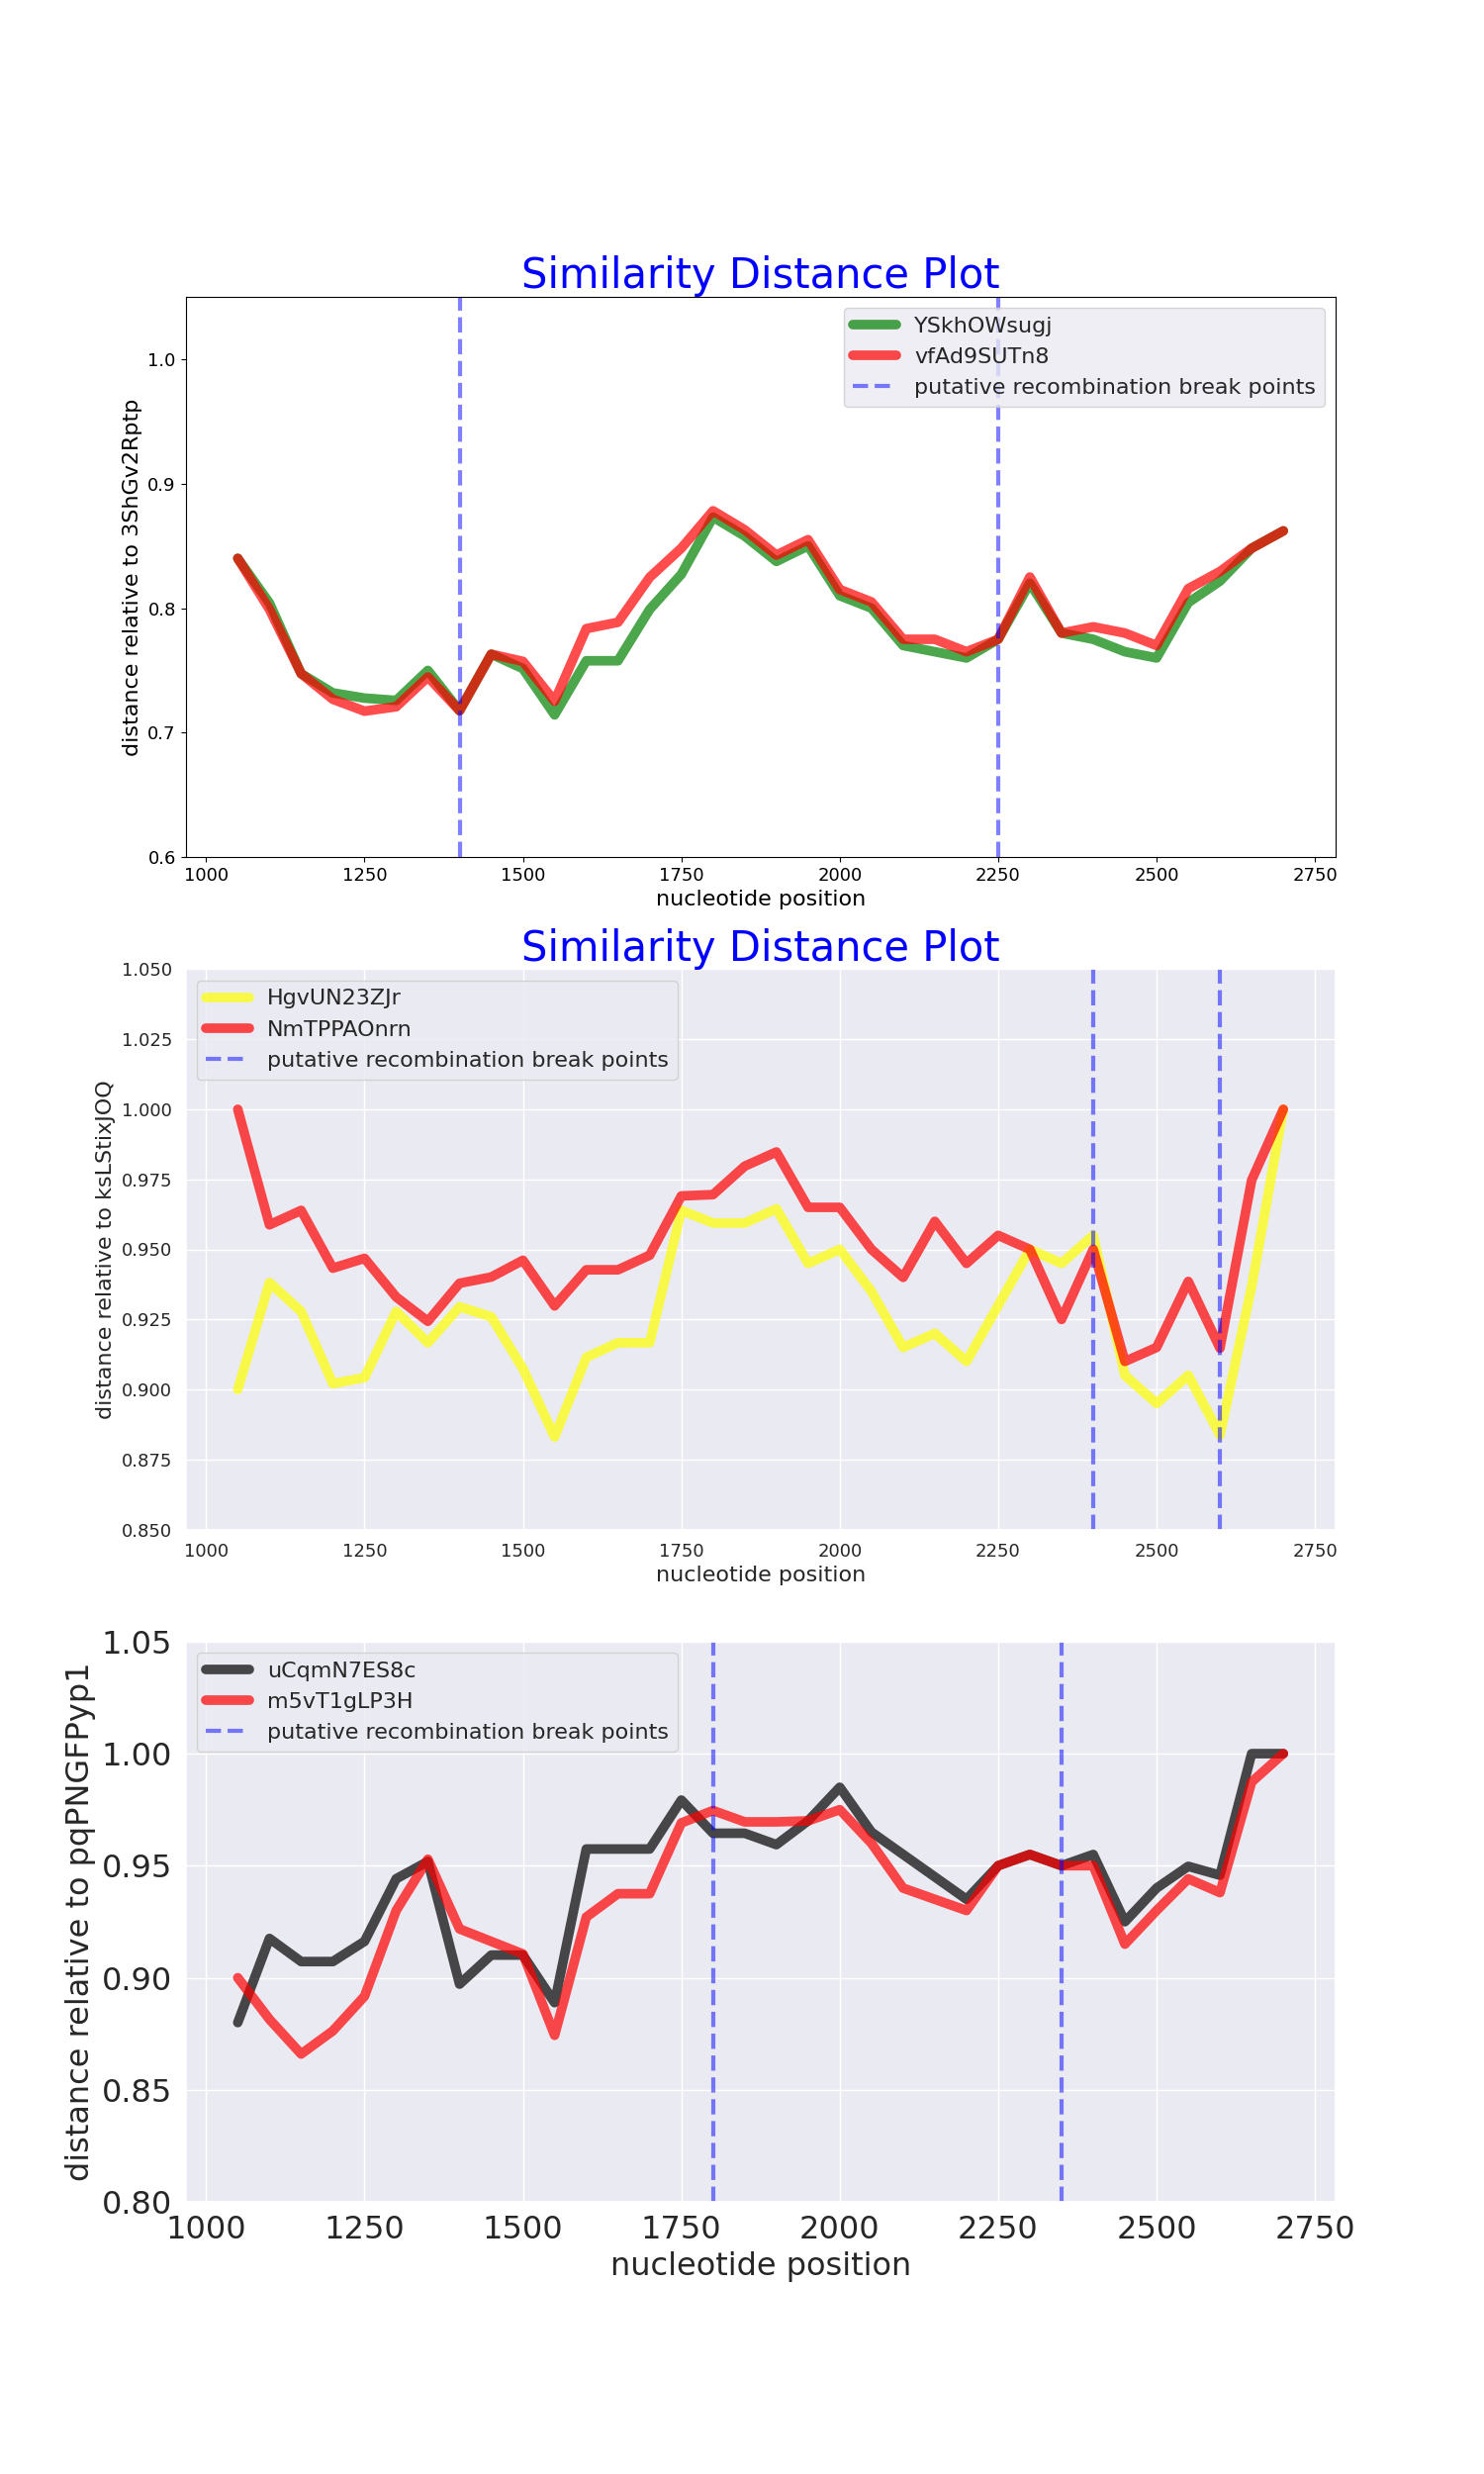
\includegraphics[width=1.0\textwidth]{hiv_plots.png}
    \caption{Breakpoints of HIV}
    \label{Figure:2}
\end{figure}

\begin{figure}
    \centering
    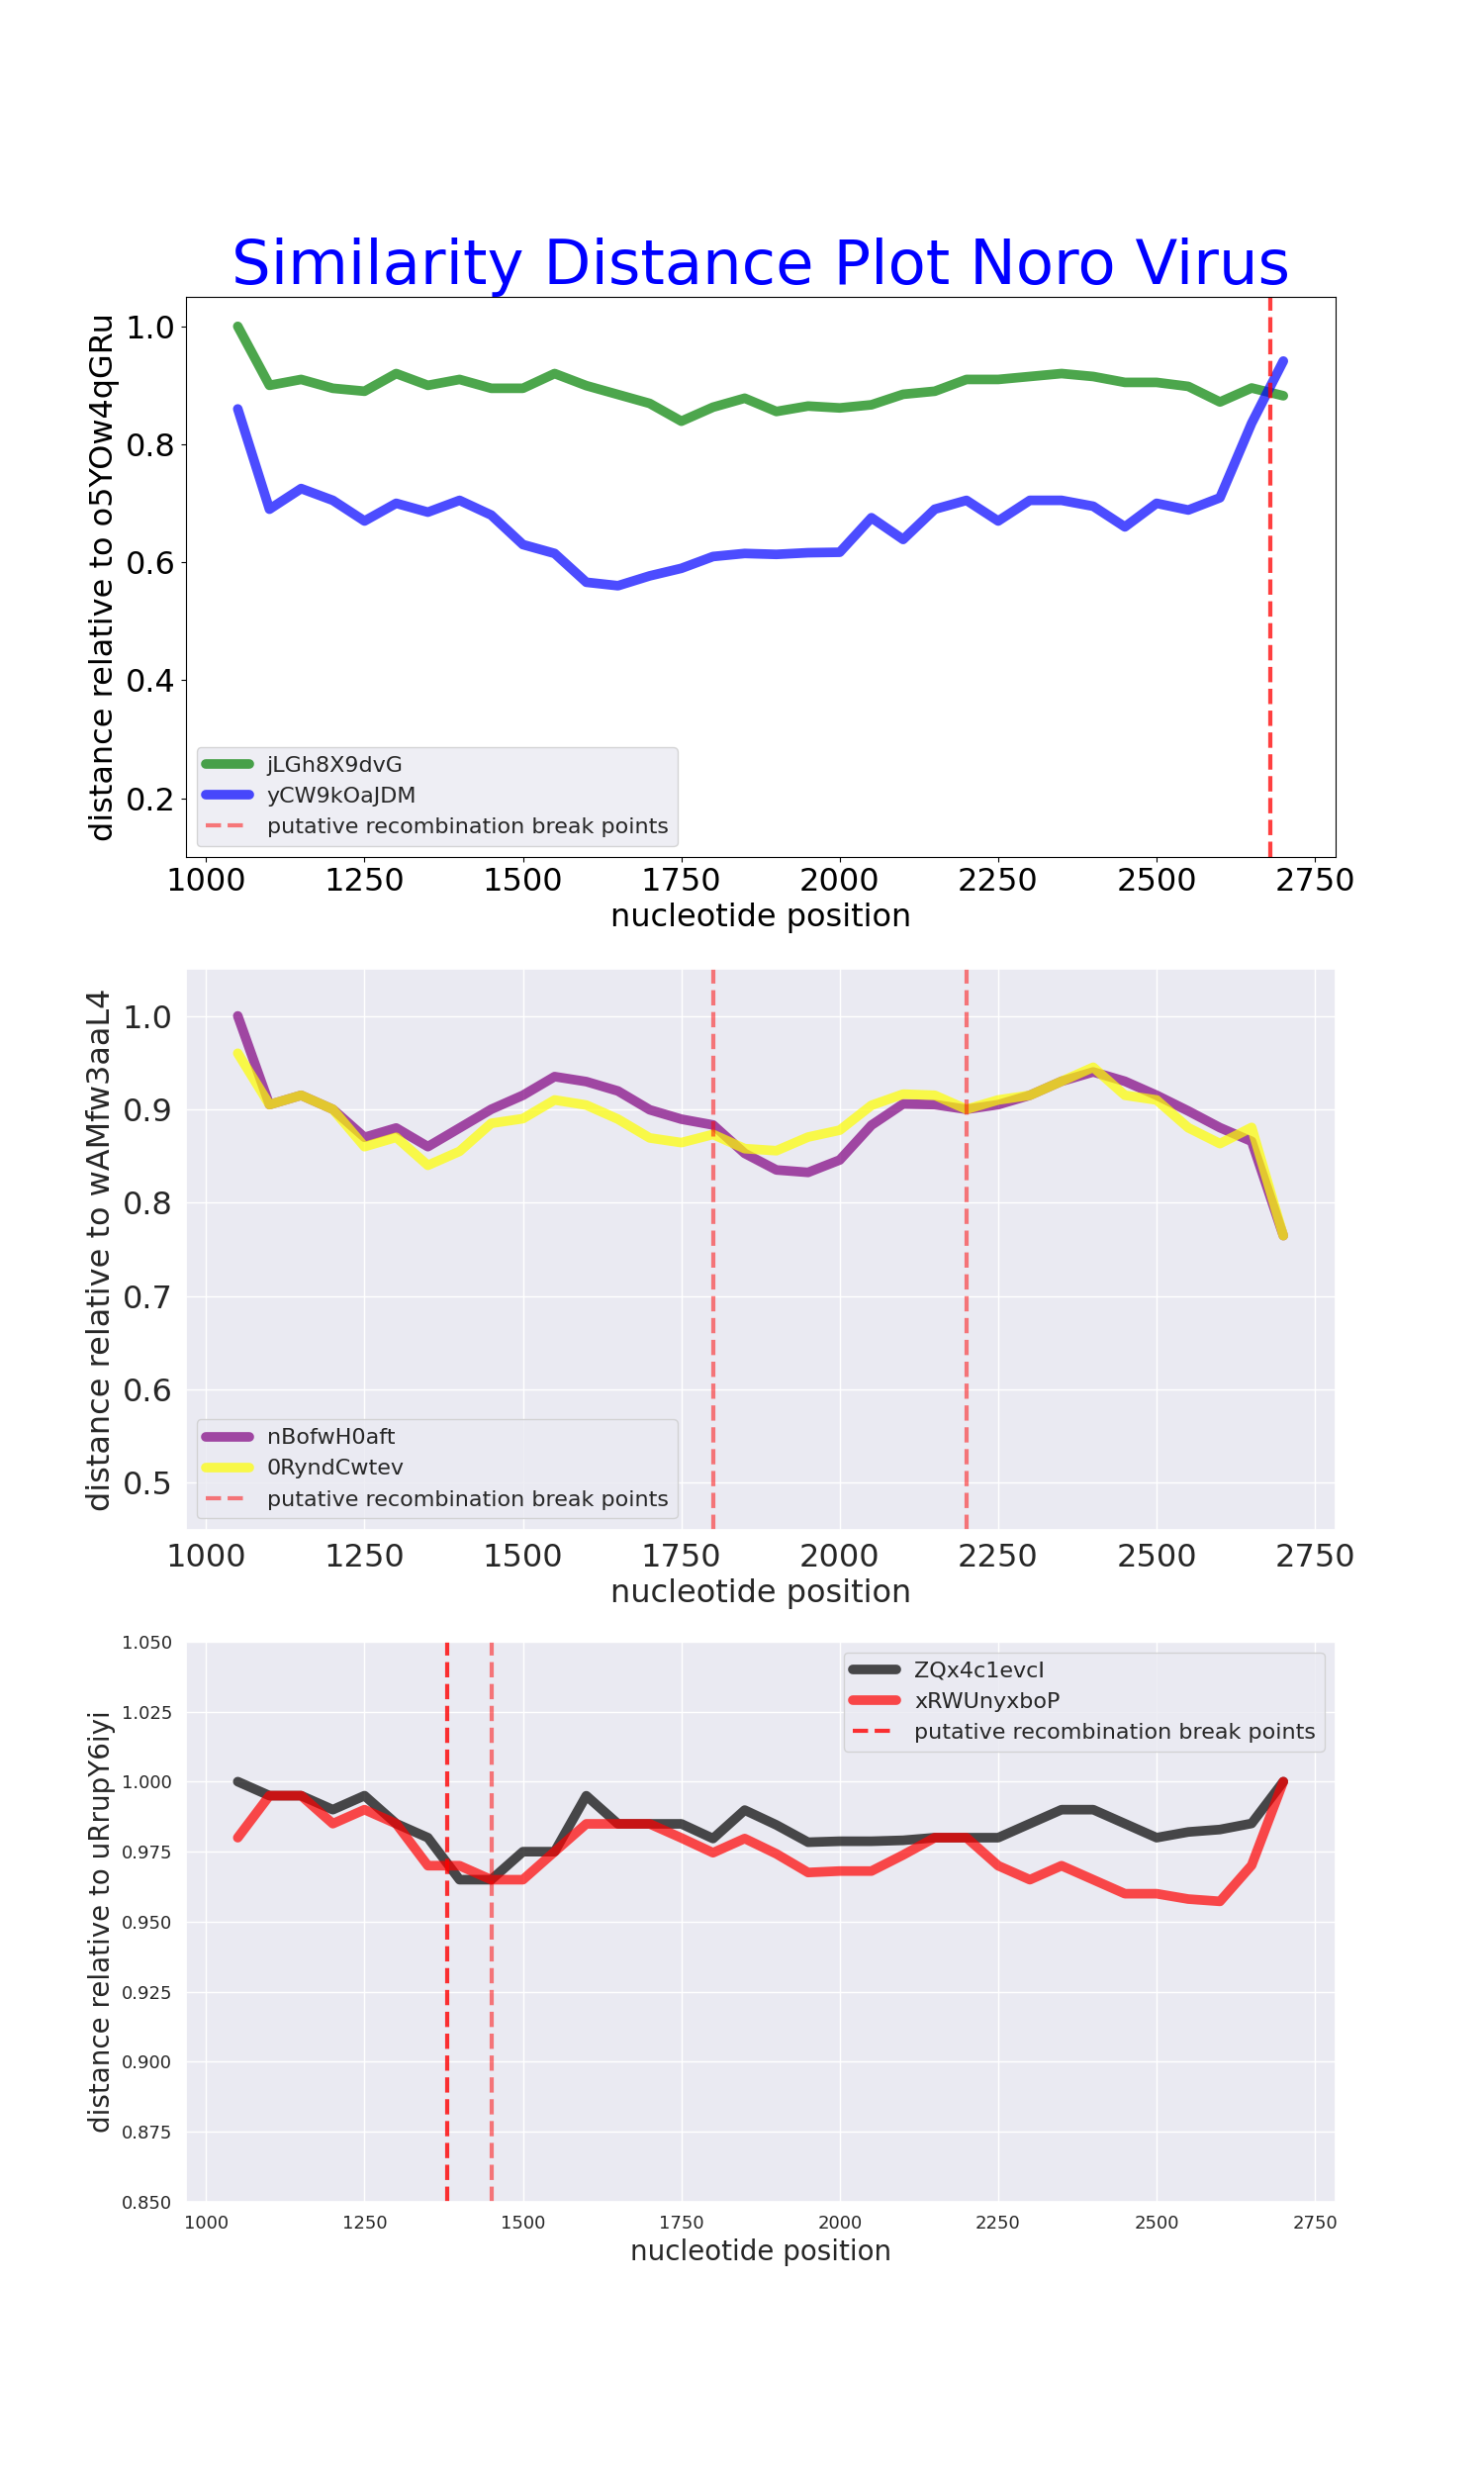
\includegraphics[width=1.0\textwidth]{noro_plots.png}
    \caption{Breakpoints of noro virus}
    \label{Figure:3}
\end{figure}

\begin{tabular}{ |p{3cm}||p{3cm}}
 \hline
 Compared Sequences of HIV& Breakpoints \\
 \hline
 (YSkhOWsugj and vfAd9SUTn8)  & At 1400 and 2350   \\
 (HgvUN23ZJr and NmTPPAOnrn)& At 2450 and 2400 \\
(uCqmN7ES8cand m5vT1gLP3H)  &At 1350 and 1500 \\
 \hline
 \label{Table:1}
\end{tabular}


\begin{tabular}{ |p{3cm}||p{3cm}}
 \hline
 ComparedSequences 0f Noro Virus & Breakpoints \\
 \hline
 (jLGh8X9dvG and yCW9kOaJDM)  & ----   \\
 (nBofwH0aft and 0RyndCwtev)& At 1800 and 2200 \\
(uCqmN7ES8c and m5vT1gLP3H)  &At 1380 and 1450 \\
 \hline
 \label{Table:2}
\end{tabular}

\subsection{FASTA Sequence Plotting}
The FASTA sequences of genomes can be visualized in several ways. We can make use of the Biopython package of renac for plotting the sequence of BCRA1 gene having multiple sequences.The Figure\ref{fig:4} shows the line plot and  Figure\ref{figu:4} shows the histogram of BCRA1 gene.

One of the most commonly used analytical data to compare different sequence is GC Percentage. In genetics and molecular biology, GC content(or guanine-cytosine content) is the s the percentage of nitrogenous bases in a DNA or RNA molecule that are either guanine (G) or cytosine (C)\cite{protozanova2006base}.The GC percentage indicates the proportion of 
bases out of an implied four total bases, also including adenine and thymine in DNA and adenine and uracil in RNA.Figure\ref{Figure:5}shows the GC percentage of BCRA1 gene.

\begin{figure}
\centering
\begin{subfigure}{.6\textwidth}
  \centering
  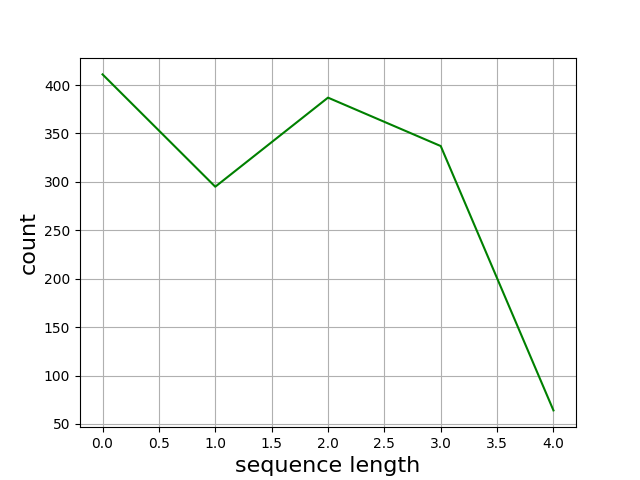
\includegraphics[width=.4\linewidth]{line_plot.png}
  \caption{A.Lineplot}
  \label{fig:4}
\end{subfigure}%
\begin{subfigure}{.6\textwidth}
  \centering
  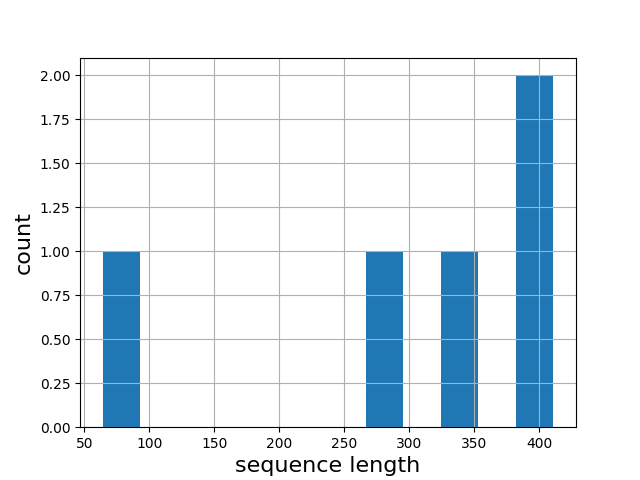
\includegraphics[width=.4\linewidth]{hist.png}
  \caption{B.Histogram}
  \label{figu:4}
\end{subfigure}
\label{figure:4}
\end{figure}

\begin{figure}
    \centering
    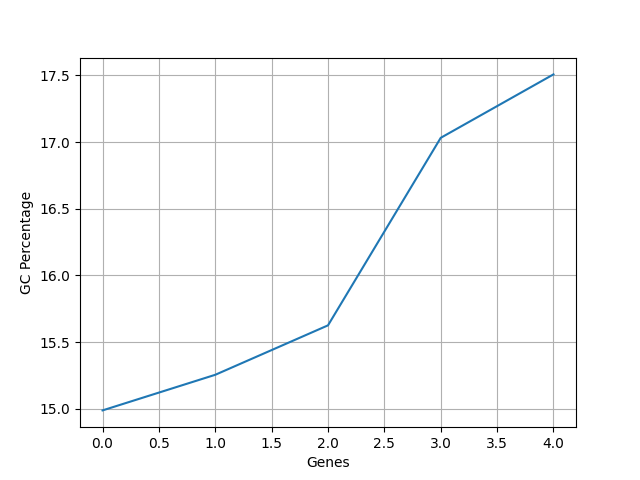
\includegraphics[height=5cm]{gcplot.png}
    \caption{GC Content}
    \label{Figure:5}
\end{figure}

\section{Conclusion:}
We can make use of the python package recan for finding the breakpoints of genomes, which is an important parameter for studying further about the recombination events. Here we found that, for Lumpy skin diseases virus's genome has breakpoints at nucleotide positions 1500 and around 1800. The breakpoints of selected HIV and Norovirus sequences are identified, which can be utilized for further studies of recombination in those sequences. Also we can plot the fasta sequences using the Bio-python package.


\bibliography{rsc.bib} 
\bibliographystyle{unsrt}

\end{document}
